%%%%%%%%%%%%%%%%%%%%%%%%%%%%%%%%%%%%%%%%%
% Beamer Presentation
% LaTeX Template
% Version 1.0 (10/11/12)
%
% This template has been downloaded from:
% http://www.LaTeXTemplates.com
%
% License:
% CC BY-NC-SA 3.0 (http://creativecommons.org/licenses/by-nc-sa/3.0/)
%
%%%%%%%%%%%%%%%%%%%%%%%%%%%%%%%%%%%%%%%%%

%----------------------------------------------------------------------------------------
%	PACKAGES AND THEMES
%----------------------------------------------------------------------------------------
\documentclass{beamer}
\mode<presentation> {
\usetheme{Singapore}
\usecolortheme{orchid}
}
\usepackage{graphicx}
\usepackage{booktabs}
\usepackage{amsmath}
\usepackage{amsthm}
\usepackage{eucal}
\usepackage{amssymb}
\usepackage{mathrsfs}

%----------------------------------------------------------------------------------------
%	TITLE PAGE
%----------------------------------------------------------------------------------------

\title[PageRank]{PageRank and Random Walks on the Web}
\author{Shannon Chatha}
\date{\today}
\begin{document}
\begin{frame}
\titlepage
\end{frame}
\begin{frame}
\frametitle{Overview}
\tableofcontents
\end{frame}

%----------------------------------------------------------------------------------------
%	PRESENTATION SLIDES
%----------------------------------------------------------------------------------------

%------------------------------------------------
\section{Introduction}
%------------------------------------------------

\begin{frame}
\frametitle{Introduction}
\begin{itemize}
\item Web pages are represented as nodes on a graph
\item A web page is important if other important pages link to it
\item Markov theory can be used to solve the PageRank equation
\end{itemize}
\begin{block}{PageRank Equation}
$\boldsymbol{\pi} = \boldsymbol{\pi} \cdot \textbf{G}$
\end{block}
\end{frame}
%------------------------------------------------
\subsection{Summation Formula for PageRank}
\begin{frame}
\frametitle{Summation Formula for PageRank}
\begin{block}{PageRank Summation}
$r(P_i) = \displaystyle \sum_{P_j\in B_{P_i }} \frac{r(P_j)}{|P_j|} $
\end{block}
\begin{block}{Iterative Summation Formula}
$r_{(k+1)}P_i = \displaystyle \sum_{P_j\in B_{P_i }}\frac{r_k(P_j)}{|P_j|}$
\end{block}
\begin{itemize}
\item Initiated with \(r_0(P_i) = \frac{1}{n}\)
\end{itemize}
\end{frame}

%------------------------------------------------

\section{Matrix Representation}
\subsection{Hyperlink Matrix}
\begin{frame}
\frametitle{Hyperlink Matrix}
\begin{block}{Hyperlink Matrix}
$\boldsymbol{H_{ij}} = \begin{cases} \frac{1}{P_j} & P_j\in B_{P_i } \\ 0 & otherwise\end{cases} $
\end{block}
\begin{example}
\begin{columns}[c]
\column{.3\textwidth} % Left column and width
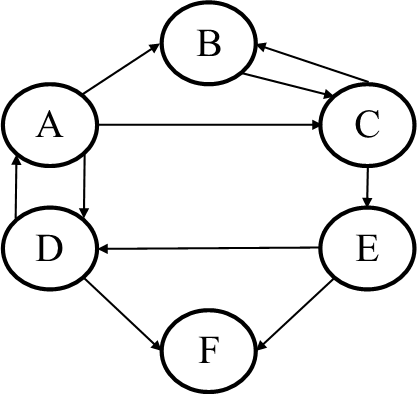
\includegraphics[width=4cm]{Picture2.png}
\column{.5\textwidth} % Right column and width
\[\textbf{H} = \left[
\begin{array}{cccccc}
0 & \frac{1}{3} & \frac{1}{3} &\frac{1}{3} & 0& 0 \\
0 & 0 & 1 & 0 & 0 & 0\\
0 & \frac{1}{2} & 0 & 0 & \frac{1}{2} & 0\\
\frac{1}{2} & 0 & 0 & 0 & 0 & \frac{1}{2}\\
0 & 0 & 0 & \frac{1}{2} & 0 &\frac{1}{2} \\
0 & 0 & 0 & 0 & 0 & 0 \\
\end{array}
\right]	
\]

\end{columns}
\end{example}
\end{frame}

%------------------------------------------------
\subsection{Modifications}
\begin{frame}
\frametitle{Modifications}
\begin{itemize}
\item Matrix will converge if it is \textbf{stochastic and primitive}
\item '\textbf{Rank Sinks}' can be solved by a '\textbf{random surfer}'
\item \textbf{Stochasticity adjustment} - rows of 0's are changed to rows of \(\frac{1}{n}\), this forms the Stochastic Matrix \textbf{S}
\item \textbf{Primitivity adjustment} - random surfer follows \textbf{S} with probability \(\alpha\), but can jump to a random page with probability \(1-\alpha\), forming the Google Matrix \textbf{G}
\end{itemize}

\end{frame}
%------------------------------------------------

\subsection{Stochastic Matrix}
\begin{frame}
\frametitle{Stochastic Matrix}
\begin{block}{Stochastic Matrix}
$\textbf{S} = \textbf{H} + \textbf{a}(\frac{1}{n}\cdot 1^{T} )$
\end{block}
\begin{example}
\[\textbf{S}=\left[
\begin{array}{cccccc}
0 & \frac{1}{3} & \frac{1}{3} &\frac{1}{3} & 0& 0 \\
0 & 0 & 1 & 0 & 0 & 0\\
0 & \frac{1}{2} & 0 & 0 & \frac{1}{2} & 0\\
\frac{1}{2} & 0 & 0 & 0 & 0 & \frac{1}{2}\\
0 & 0 & 0 & \frac{1}{2} & 0 &\frac{1}{2} \\
\frac{1}{6} & \frac{1}{6} & \frac{1}{6} & \frac{1}{6} & \frac{1}{6} & \frac{1}{6} \\
\end{array}
\right]	
\]
\end{example}
\end{frame}
%------------------------------------------------

\subsection{Google Matrix}
\begin{frame}
\frametitle{Google Matrix}
\begin{block}{Google Matrix}
$\textbf{G} = \alpha\textbf{S} + (1-\alpha)\cdot\frac{1}{n}\cdot 1^{T}$
\end{block}
\begin{example}
\[\textbf{G}=0.85\textbf{S} + 0.15\cdot\frac{1}{6}\cdot\left(
\begin{array}{cccccc}
1&1&1&1&1&1\end{array}
\right)
\]
\[\textbf{G}=\left[
\begin{array}{cccccc}
0.025 & 0.308 & 0.308 & 0.308 & 0.025 & 0.025 \\
0.025 & 0.025 & 0.875 & 0.025 & 0.025 & 0.025\\
0.025 & 0.450 & 0.025 & 0.025 & 0.450 & 0.025\\
0.450 & 0.025 & 0.025 & 0.025 & 0.025 & 0.450\\
0.025 & 0.025 & 0.025 & 0.450 & 0.025 &0.450 \\
0.166 & 0.166 & 0.166 & 0.166 & 0.166 & 0.166 \\
\end{array}
\right]	
\]
\end{example}
\end{frame}
%------------------------------------------------
\section{Solving the Matrix}
\subsection{Power Method}
\begin{frame}
\frametitle{Power Method}
\begin{itemize}
\item Solve the PageRank equation by finding an eigenvector of \textbf{G} with eigenvalue 1
\end{itemize}
\begin{block}{Power Method}
$\boldsymbol{\pi^{(k+1)}} = \boldsymbol{\pi^{(k)}}\cdot \textbf{G}$
\end{block}
\begin{columns}[c]
\column{.5\textwidth} % Left column and width
\begin{itemize}
\item Basic principle: $\boldsymbol{\pi^{(k+1)}}$ will converge to a stationary vector
\item Initiated with $\boldsymbol{\pi_{0}} = \frac{1}{n}$
\item Slow but has many advantages
\end{itemize}

\column{.5\textwidth} % Right column and width
\begin{example}
\[\boldsymbol{\pi}=\left[
\begin{array}{c}
0.116\\ 
0.308\\ 
0.308\\ 
0.308\\ 
0.025\\
0.025 \\
\end{array}
\right]	
\]
\end{example}
\end{columns}
\end{frame}

%------------------------------------------------

\section{Summary}
\begin{frame}
\frametitle{Summary}
\begin{itemize}
\item A web pages importance is reliant on other pages linking to it
\item \textbf{G} is formed due to modifications on \textbf{H} and \textbf{S}
\item Solve the PageRank equation using the power method to find a stationary vector \(\boldsymbol{\pi}\)
\end{itemize}
\end{frame}

%-------------------------------------------
\begin{frame}
\frametitle{Questions?}
\begin{block}{References}
[1] Google’s PageRank and Beyond: The Science of Search Engine Rankings, A. N. Langville and C. D. Meyer, 2006

[2] A Course on the Web Graph, A. Bonato, 2008

[3]How Google Finds Your Needle in the Web’s Haystack, D. Austin, 2006 

[4] Introduction to Information Retrieval, C. D. Manning, P. Raghavan, H. Sch\"utze, 2008 \end{block}
\end{frame}
%----------------------------------------------------------------------------------------

\end{document} 